% !TEX root = ../main.tex
\section{Winged Kin}
\begin{linenumbers}
\DndDropCapLine{Y}{es, sure, you can create a machine to}
\textit{glide.
You can even ride a creature to stay aloft.
But you will never truly fly.
No kin can tame the sky with such grace as the irds.
Trust me, if they weren't so humble as to live among us, constrained to the ground, we'd be building temples to venerate their graciousness.}

\hspace*{\fill} --- Josiah, priest from the church of Rhekesh.

Sequestered in high mountains, deep jungles, and hot deserts, the irds, sisz rlue, or winged kin are known to survive some of the harshest environments all around Yuadrem.

\subsection*{Beak and Feather}
From below, irds look much like large birds.
Only when they descend to roost or walk in the ground does their humanoid appearance reveal itself.
Standing upright, an ird might reach 2 meters tall.
They have long, narrow legs that taper to sharp talons.

Feathers cover their bodies, with their plumage typically reflecting the environment they develop in.
Their heads complete the avian appearance, being that of a parrot, hawk, or vulture.
Irds' arms have very long feathers, which allow them to fly with ease.
The three subraces of the irds are very distinct from each other.
This is due to the fact that they were created by three different ets, all in pursuit of a same goal, yet for different environments.

The winged kin are the only gendered species created by the tall kin.
Some time after reproduction, a female will lay one to three eggs and the couple will refrain from contact with others in their tribe, becoming extremely protective of their children until they reach maturity.

\subsection*{Sky Wardens}
Nowhere are the irds more comfortable than in the sky.
They can spend hours in the air, and some go as long as days, locking their wings in place and letting the thermals hold them aloft.
In battle, they prove dynamic and acrobatic fliers, moving with remarkable speed and grace, diving to lash opponents with weapons or talons before turning and flying away.

Once airborne, an ird leaves the sky with reluctance.
They sometimes forget or ignore vertical distances, and they have nothing but pity for those earthbound kins forced to live and toil constrained to the ground.

The ird are a tribal species, and its rare for a tribe to hold more than a hundred irds at once.
The only exceptions to this rule are the Krudzal and Kaldrathal, both large countries in the northern reaches of Yuadrem.
They are welcoming to traders and visitors in general, but generally don't allow members from other kins to be permanent residents within their territory, and frown upon guests who overstay their welcome.

Once tribes of irds settle in an area, they share a hunting territory that extends across an area up to 150 km on a side, with each tribe hunting in the lands nearest to their colony, ranging farther should game become scarce.
A typical colony consists of one large, open-roofed nest made of woven vines.
The eldest acts as leader with the support of a shaman.

\subsection*{Avian Mannerisms}
The resemblance of ird to birds isn't limited to physical features.
Irds display many of the same mannerisms as ordinary birds.
They are fastidious about their plumage, frequently tending their feathers, cleaning and scratching away any tiny passengers they might have picked up.
When they deign to descend from the sky, they often do so near pools where they can catch fish and bathe themselves.
Even when perched on a high branch or at rest in their mountaintop homes, they appear alert, with eyes moving and bodies ready to take flight.

Many winged kin punctuate their speech with chirps, sounds they use to convey emphasis and to shade meaning.
An ird might become frustrated with people who fail to pick up on the nuances; an ird's threat might be taken as a jest and vice versa.
Confinement terrifies the winged kin.
To be imprisoned by the cold, unyielding earth is a torment few ird can withstand.

\subsection*{Innate Curiosity}
Irds are naturally curious which, summed with their freedom of movement, leads to them being the ideal explorers and adventurers.
They use their large wings to travel to almost any place in the entirety of Yuadrem, and as such they've become a common sight in all its reaches.
Outside of their tribes, irds do enjoy living within other civilizations, and its rare to see a city or large settlement without at least one ird inhabitant.

Winged kin tribes are accepting of their members leaving for indefinite amounts of time, and this is even encouraged in many communities.
In fact, the population of a tribe is ever-changing, with the only constants being the eldest members and the shaman.
This means that neighboring tribes have strong and healthy relations, each coming to aid the ones in need without question.
Another consequence of their tendency to travel is the versatility of ird artisans, who integrate techniques from all around Yuadrem into their craft.

\subsection*{Ird Names}
Ird names separate into two main categories.
The first resemble their original language, Harualish, and include clicks, trills, and whistles to the point that other kins have a difficult time pronouncing them.
When interacting with other races, they may use nicknames gained from people they meet or shortened forms of their full names.

On the other hands, irds from Krudzal, Kaldrathal, and other civilized lands tend to speak Shanise.
Shanise is a language formed from the interaction of Harualish-speaking irds and Avshenese-speaking gats in the north.

An ird last name is usually simply ``son/daughter of'' followed by one of their parent's name.
Most irds admire their parents, and wear their last names with pride.

\paragraph{Harualish Ird Names} Aera, Aial, Aur, Deekek, Errk, Heehk, Ikki, Kleeck, Oorr, Ouss, Quaf, Quierk, Salleek, Urreek, Zeed.

\paragraph{Male Shanise Ird Names} Aden, Azat, Daneal, Dirkir, Eastean, Goker, Idrahin, Jakod, Jaldor, Jasin, Kuneit, Lutdzu, Nuretin, Nutlar, Rezat, Semir, Shasar, Tajik, Tenel, Tshasin, Unut.

\paragraph{Female Shanise Ird Names} Aise, Asutshan, De\~na, Dilsad, Dorun, Drinja, Eda, Gudlag, Gulden, Hazal, Iris, Katrin, Kisnet, Naina, Nerhe, Sehil, Selna, Sher, Solveag, Tedziye, Zainej.

\subsection*{Traits}
Your ird character has access to different abilities common to all subraces:

\subparagraph{Ability Score Increase} Your Dexterity score increases by 1, and your Wisdom score increases by 1.

\subparagraph{Age} Ird reach maturity by age 14, and don't usually live much longer than 150 years.

\subparagraph{Alignment} Ird have an inclination towards the red tide, which is supported by their adventurous lifestyle.

\subparagraph{Size} Ird are tall, and range from 1.70 to 2 meters.
They have thin bodies and hollow bones, weighing between 40 and 50 kilograms.
Your size is medium.

\subparagraph{Speed} You have a walking speed of 7.5 meters, and a flying speed of 15 meters.
To fly, you can't wear medium or heavy armor, carry heavy weapons, wield a shield or be encumbered.
Since you flap your arms to fly, you cannot use them to attack while flying.
You can use your versatile talons to hold and use simple weapons or spellcasting foci.

\subparagraph{Graceful Landing} Your years of living at great heights have taught you how to fall more gracefully.
You reduce the damage die for fall damage from a d6 to a d4, and you do not fall prone after taking falling damage, unless you are unconscious.

\subparagraph{Keen Senses} You are competent in the Perception skill.

\subsubsection{Qulbaba Ird}
Many irds can be found living in isolated tribes inside the jungles of Yuadrem.
In the east they live in Harual, and in the west in the Jenkashian empire.
Qulbaba ird have a face resembling that of a parrot, and their feathers' coloration depends on their gender.
Males usually have very brightly colored feathers, showing any combination of colors.
Females mostly have dull gray, brown, and dark green feathers, aiding their ability to hide in the jungle.

\subparagraph{Ability Score Increase} Your time gliding between branches and vines has augmented your flying capacity.
Your Dexterity score increases by 1.

\subparagraph{Bright Coloration} As a male, you are competent in the Performance skill.
Additionally, you have advantage on Charisma (Intimidation) checks made against creatures with an Intelligence score of 5 or less.

\subparagraph{Dark Feathers} As a female, you have advantage in Dexterity (Stealth) checks made in dim or dark light or in heavily forested areas.

\subparagraph{Strong Talons} You are competent with unarmed strikes, which deal 1d4 plus your Dexterity modifier as slashing damage on a hit.
Additionally, you have advantage of Strength (Athletics) checks made to climb any surface your talons could reasonably grip.

\begin{figure}[!b]
    \centering
    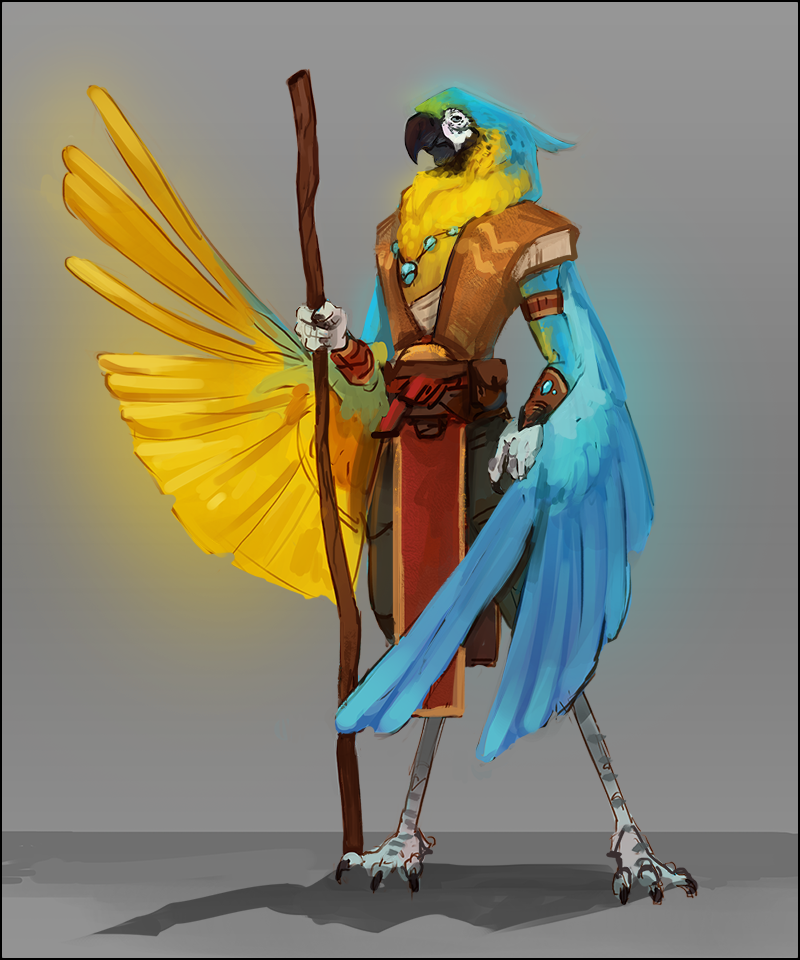
\includegraphics[width=0.48\textwidth]{02kins/img/12ird_qulbaba.png}
\end{figure}

% \newpage

\subsubsection{Thulkraka Ird}
Unlike their brethren, the Thulkraka tribes that settled on the many mountaintops of Yuadrem live their lives mostly constrained to the ground, and are only able to fly when the harsh mountain weather allows it.
They are thus bulkier than the average ird, and commonly are clumsy fliers due to their lack of experience.
Their faces are similar to that of hawks, and their feathers' coloration is bleak and cold, usually sporting white, gray, light blue, and brown colors.

\subparagraph{Ability Score Increase} Isolated from other races, you have been able to take the time to truly appreciate the calmness of the mountains.
Your Wisdom score is increased by 1.

\subparagraph{Bulky Frame} Your flying speed is reduced to 10.5 meters, but you can fly while carrying heavy weapons and/or wearing medium armor.

\subparagraph{Mountain Born} You're acclimated to altitudes up to 6,000 meters.
You're also naturally adapted to cold climates.

\subparagraph{Thulkrakian Descent} You are competent with smith's tools, as is tradition amongst your people.

\begin{figure}[!t]
    \centering
    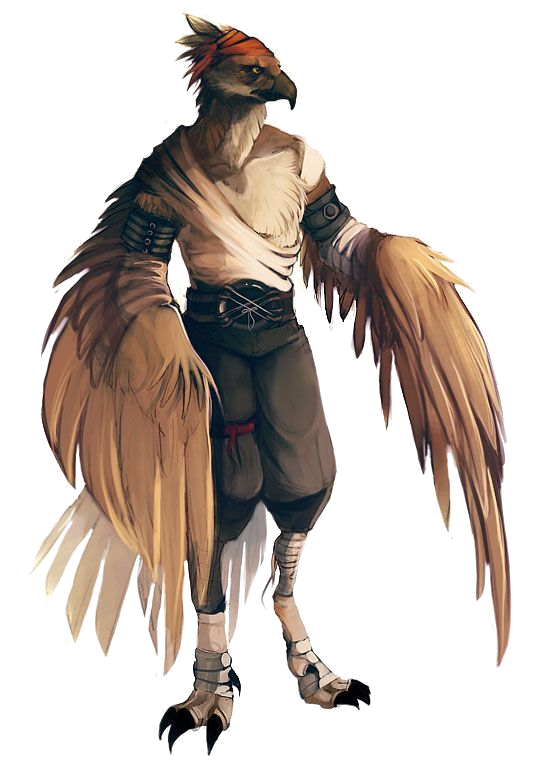
\includegraphics[width=0.47\textwidth]{02kins/img/12ird_thulkraka.png}
\end{figure}

\subsubsection{Dratl Ird}
Irds from the Dratl houses are known as ruthless ruffians, and are pariahs to the other winged kin subspecies.
They are known for constantly harassing the other ird tribes, as well as any who approach their territory.
The are collectively banned from entering any tribe from the other subspecies, and are usually unwelcome in towns and cities due to their bad reputation.

Nowadays, Dratl houses are scattered around the Zoedrem desert, mostly unorganized.
These are the remnants of the once great empire of Hulnar, disbanded in 591 AS.
Despite their lost grandness, they are still feared by the common people, and continue to fiercely protect their hunting grounds.

A Dratl ird's beak resembles that of a vulture, and their feathers are generally black, white, and red.
As a dratl ird grows up, their irises become noticeably white, while the sclera surrounding them turn into a bright red color.

\subparagraph{Ability Score Increase} Your time surviving in the harsh climate of the desert has given you an increased robustness.
Your Constitution score is increased by 1.

\subparagraph{Wing Flap} When you use the disengage action, you can choose to use another action to propel yourself upward a distance equal to half your flying speed.

\subparagraph{Bone Breaker} While flying, you can attempt to attack a creature with an eviscerating attack.
Using two actions, you can swoop down up to your flying speed towards a creature you can see, and make a melee weapon attack roll against it.
If the attack hits, it's a critical hit.
The attack is tiring, and you can use this trait only once per combat encounter.

\begin{figure}[!b]
    \centering
    \includegraphics[width=0.47\textwidth]{02kins/img/12ird_dratl.png}
\end{figure}
\end{linenumbers}

\newpage
